% -----------------------------------------------------------------
% Document class: Article
\documentclass[ a4paper, twoside, 11pt]{article}
\usepackage{../../../macros-general}
\usepackage{../../../macros-article}
% Number of the handout, quiz, exam, etc.
\newcommand{\numero}{01}
\setcounter{numero}{\numero}

% -----------------------------------------------------------------
\begin{document}
\allowdisplaybreaks

\begin{center}
\Large Mec\'anica Vectorial (MECG-1001): Lecci\'on \numero \\[2ex]
\small \textbf{Semestre:} 2017-2018 T\'ermino II \qquad
\textbf{Instructor:} Luis I. Reyes Castro \qquad
\textbf{Paralelo:} 09
\end{center}
\fullskip

% =============================================
\begin{problem}
Para la armadura mostrada en la siguiente figura:

\begin{figure}[htb]
\centering
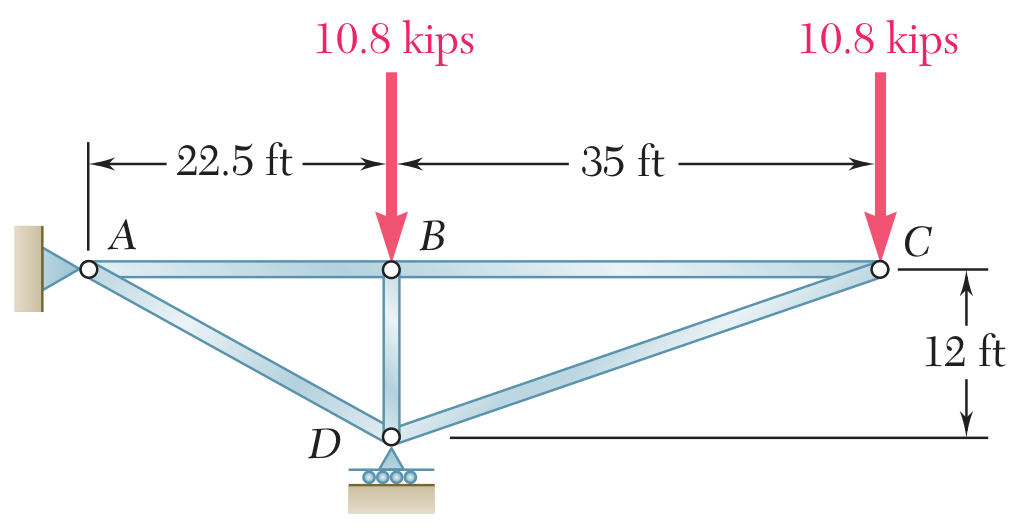
\includegraphics[width=0.56\textwidth]{prob-armadura.jpg}
\end{figure}

\begin{enumerate}[label=\textbf{\alph*)}]
\item \textbf{3 Puntos:} Encuentre las reacciones en $A$ y $D$. \\[1ex] \emph{Soluci\'on:}
\begin{align*}
\sum F_x \; \colon \; & A_x \; = \; 0 \text{ kips} \\[1ex]
\sum F_y \; \colon \; & A_y + D_y \; = \; 21.6 \\[1ex]
\sum M_A \; \colon \; & +22.5 \cdot ( D_y - 10.8 ) - 57.5 \cdot (10.8) \; = \; 0 \\[1ex]
& \Longrightarrow \; D_y \; = \; +38.4 \text{ kips},
\; A_y \; = \; -16.8 \text{ kips}
\end{align*}
\item \textbf{4 Puntos:} Escriba las ocho ecuaciones asociadas con los cuatro nodos de la armadura, denotando compresi\'on con signo positivo y tensi\'on con signo negativo. \\[1ex] \emph{Soluci\'on:} Primero definimos: 
\[
\theta_{AD} \; = \; \arctan( 12 / 22.5 ) \; = \; 28.07\deg \qquad \qquad
\theta_{CD} \; = \; \arctan( 12 / 35 ) \; = \; 18.92\deg
\]
Nodo $A$: 
\begin{align*}
\sum F_x \; \colon \; & -F_{AB} -F_{AD} \, \cos(\theta_{AD}) \; = \; 0 \\[1ex]
\sum F_y \; \colon \; & +F_{AD} \, \sin(\theta_{AD}) \; = \; +16.8
\end{align*}
Nodo $B$: 
\begin{align*}
\sum F_x \; \colon \; & +F_{AB} -F_{BC} \; = \; 0 \\[1ex]
\sum F_y \; \colon \; & +F_{BD} \; = \; +10.8
\end{align*}
Nodo $C$: 
\begin{align*}
\sum F_x \; \colon \; & +F_{BC} + F_{CD} \, \cos(\theta_{CD}) \; = \; 0 \\[1ex]
\sum F_y \; \colon \; & +F_{CD} \, \sin(\theta_{CD}) \; = \; +10.8
\end{align*}
Nodo $D$: 
\begin{align*}
\sum F_x \; \colon \; & +F_{AD} \, \cos(\theta_{AD}) - F_{CD} \, \cos(\theta_{CD}) \; = \; 0 \\[1ex]
\sum F_y \; \colon \; & -F_{AD} \, \sin(\theta_{AD}) - F_{BD} - F_{CD} \, \sin(\theta_{CD}) \; = \; -38.4
\end{align*}

\item \textbf{2 Puntos:} Calcule la fuerza interna en cada eslab\'on. \\[1ex] \emph{Soluci\'on:} Primero, del Nodo $A$ obtenemos: 
\[
F_{AD} \; = \; +35.7 \text{ kips}
\qquad \Longrightarrow \qquad
F_{AB} \; = \; -31.5 \text{ kips}
\]
Luego, del Nodo $B$ obtenemos: 
\[
F_{BC} \; = \; -31.5 \text{ kips}
\qquad \qquad
F_{BD} \; = \; +10.8 \text{ kips}
\]
Finalmente, del Nodo $C$ obtenemos: 
\[
F_{CD} \; = \; +33.3 \text{ kips}
\]
\end{enumerate}

\end{problem}
\fullskip

% =============================================
\begin{problem}
Para el armaz\'on mostrado en la siguiente figura:

\begin{figure}[htb]
\centering
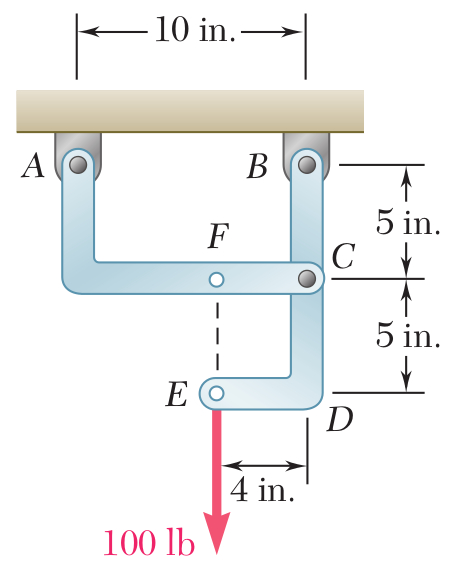
\includegraphics[width=0.28\textwidth]{prob-armazon.jpg}
\end{figure}

\begin{enumerate}[label=\textbf{\alph*)}]
\item \textbf{2 Puntos:} Bosqueje los diagramas de cuerpo libre correspondientes. \\[1ex] \emph{Soluci\'on:}
\begin{itemize}
\item Cuerpo $AFC$: 
\begin{align*}
\sum F_x \; \colon \; & A_x - C_x \; = \; 0 \\[1ex]
\sum F_y \; \colon \; & A_y - C_y \; = \; 0 \\[1ex]
\sum M_A \; \colon \; & -5 \cdot C_x -10 \cdot C_y \; = 0
\end{align*}
\item Cuerpo $BCDE$: 
\begin{align*}
\sum F_x \; \colon \; & B_x + C_x \; = \; 0 \\[1ex]
\sum F_y \; \colon \; & B_y + C_y \; = \; 100 \\[1ex]
\sum M_B \; \colon \; & +5 \cdot C_x - 4 \cdot 100 \; = 0
\end{align*}
\end{itemize}

\item \textbf{2 Puntos:} Calcule la fuerza que la barra $AFC$ ejerce sobre la barra $BCDE$ en $C$. \\[1ex] \emph{Soluci\'on:} Resolviendo en el cuerpo $BCDE$ la sumatoria de momentos en $B$ para $C_x$ obtenemos: 
\[
C_x \; = \; +80 \text{ lb}
\]
Finalmente, resolviendo en el cuerpo $AFC$ la sumatoria de momentos en $A$ para $C_y$ obtenemos: 
\[
C_y \; = \; -40 \text{ lb}
\]

\item \textbf{2 Puntos:} Calcule las reacciones en $A$ y $B$. \\[1ex] \emph{Soluci\'on:} De las sumatorias de fuerzas en el cuerpo $AFC$ obtenemos: 
\[
A_x \; = \; C_x \; = \; +80 \text{ lb}, \qquad \qquad
A_y \; = \; C_y \; = \; -40 \text{ lb}
\]
Luego, de las sumatorias de fuerzas en el cuerpo $BCDE$ obtenemos: 
\[
B_x \; = \; -C_x \; = \; -80 \text{ lb}, \qquad \qquad
B_y \; = \; 100 - C_y \; = \; +140 \text{ lb}
\]

\end{enumerate}

\end{problem}
\fullskip

% =============================================
\begin{problem}
\textbf{4 Puntos:} Para la viga mostrada en la siguiente figura encuentre la fuerza cortante $V(x)$ y el momento flector $M(x)$ como funci\'on de la posici\'on $x \in [0,4]$. 

\begin{figure}[htb]
\centering
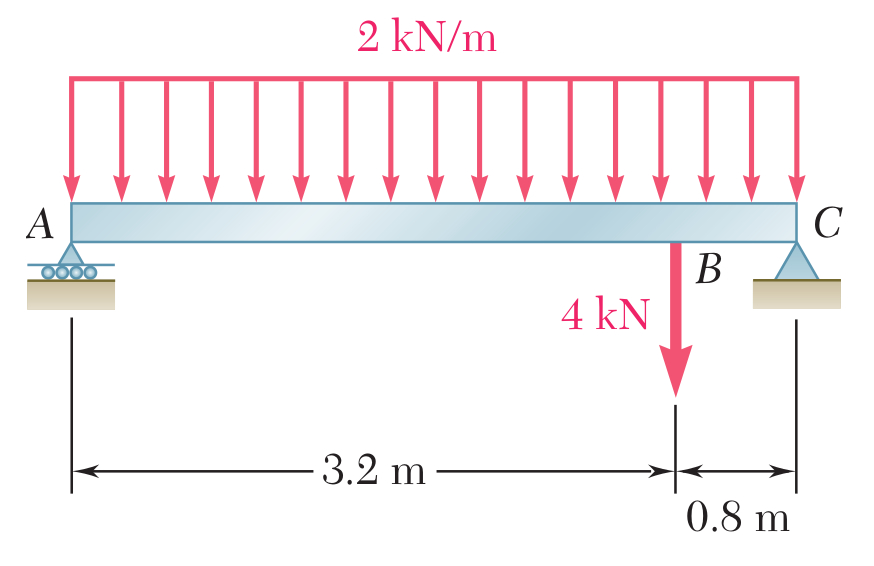
\includegraphics[width=0.42\textwidth]{prob-vigas.jpg}
\end{figure}

\emph{Soluci\'on:} Empezamos con las reacciones: 
\begin{align*}
\sum F_x \; \colon \; & C_x \; = \; 0 \text{ kN} \\[1ex]
\sum F_y \; \colon \; & A_y + C_y \; = \; 12 \\[1ex]
\sum M_A \; \colon \;
& -(1/2)(2)(4^2) - (3.2)(4) + 4 \, C_y \; = \; 0 \\[1ex]
& \Longrightarrow \;
C_y \; = \; +7.2 \text{ kN}, \qquad
A_y \; = \; +4.8 \text{ kN}
\end{align*}

Para la secci\'on donde $x \in [ \, 0, \, 3.2]$ :
\begin{align*}
\sum F_x \; \colon \; & F(x) \; = \; 0 \text{ kN} \\[1ex]
\sum F_y \; \colon \;
& +4.8 - 2 \, x - V(x) \; = \; 0
\quad \Longrightarrow \;
V(x) \; = \; -2 \, x + 4.8 \text{ kN} \\[1ex]
& \; \Longrightarrow \;
M(x) \; = \; M(0) + \int_{0}^x (-2 \, x + 4.8) \, dx
\; = \; - x^2 + 4.8 \, x \text{ kN-m} \\[1ex]
& \; \Longrightarrow \;
M(3.2) \; = \; +5.12 \text{ kN-m}
\end{align*}

Para la secci\'on donde $x \in [ \, 3.2, \, 4]$ :
\begin{align*}
\sum F_x \; \colon \; & F(x) \; = \; 0 \text{ kN} \\[1ex]
\sum F_y \; \colon \;
& +4.8 - 2 \, x - 4 - V(x) \; = \; 0
\quad \Longrightarrow \;
V(x) \; = \; -2 \, x + 0.8 \text{ kN} \\[1ex]
& \; \Longrightarrow \;
M(x) \; = \; M(3.2) + \int_{3.2}^x (-2 \, x + 0.8) \, dx \\[1ex]
& = \; +5.12 - x^2 + 0.8 \, x + 7.68 \; = \;
- x^2 + 0.8 \, x + 12.8 \text{ kN-m} 
\end{align*}

En conclusi\'on: 
\begin{itemize}
\item Fuerza cortante: 
\[
V(x) \; = \;
\begin{dcases}
-2 \, x + 4.8 \text{ kN},
& \text{para todo } x \in [ \, 0, \, 3.2] \\
-2 \, x + 0.8 \text{ kN},
& \text{para todo } x \in [ \, 3.2, \, 4] \\
\end{dcases}
\]
\item Momento flector: 
\[
M(x) \; = \;
\begin{dcases}
- x^2 + 4.8 \, x \text{ kN-m},
& \text{para todo } x \in [ \, 0, \, 3.2] \\
- x^2 + 0.8 \, x + 12.8 \text{ kN-m} ,
& \text{para todo } x \in [ \, 3.2, \, 4] \\
\end{dcases}
\]
\end{itemize}

\end{problem}
\fullskip

% =============================================
\begin{problem}
El oleoducto mostrado en la siguiente figura est\'a soportado cada 6 ft mediante suspensores verticales fijos a un cable como se muestra en la figura. Debido al peso combinado del ducto y su contenido, cada suspensor experimenta una tensi\'on de 400 lb. Si se sabe que $d_C = 12$ ft, determine: 

\begin{figure}[htb]
\centering
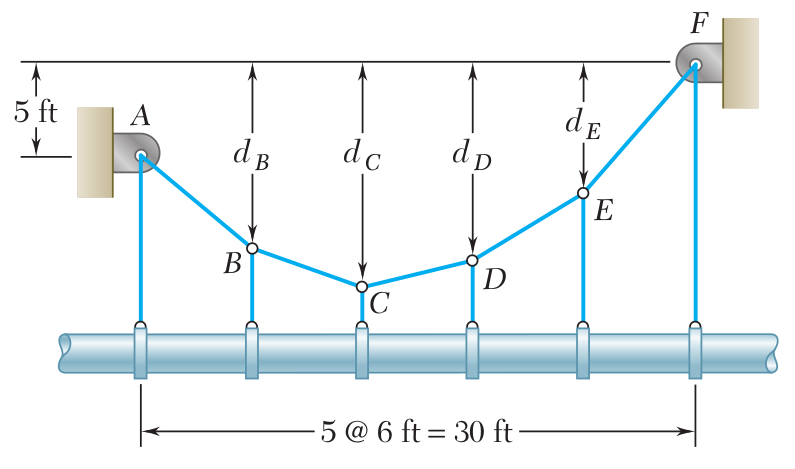
\includegraphics[width=0.52\textwidth]{prob-cables.jpg}
\end{figure}

\begin{enumerate}[label=\textbf{\alph*)}]
\item \textbf{3 Puntos:} La altura $d_B$. \emph{Nota:} Por favor ignore las cargas en $A$ y $F$. \\[1ex] \emph{Soluci\'on:} Primero consideramos el cable completo y sumamos momentos: 
\begin{align*}
\sum M_F \; \colon \;
& +(6+12+18+24)(400) + 5 \, A_x - 30 \, A_y \; = \; 0 \\[1ex]
& \Longrightarrow \;
A_x - 6 \, A_y + 4800 \; = \; 0
\; \Longrightarrow \;
A_x \; = \; 6 \, A_y - 4800 \; = \; 0
\end{align*}
Luego consideramos la secci\'on $ABC$ y sumamos momentos: 
\begin{align*}
\sum M_C \; \colon \;
& +6(400) -7 \, A_x - 12 \, A_y \; = \; 0 \\[1ex]
& \Longrightarrow \; 7 \, A_x + 12 \, A_y - 2400 \; = \; 0 \\[1ex]
& \Longrightarrow \;
A_x \; = -800 \text{ lb}, \quad A_y \; = \; +666.7 \text{ lb}
\end{align*}
Finalmente, consideramos la secci\'on $AB$ y sumamos momentos: 
\begin{align*}
\sum M_B \; \colon \;
& +( d_B - 5 )(800) - (6)(666.7) \; = \; 0 \\[1ex]
& \Longrightarrow \;
d_B \; = \; 10.0 \text{ ft}
\end{align*}

\item \textbf{2 Puntos:} Las alturas $d_D$ y $d_E$. \\[1ex] \emph{Soluci\'on:} Considerando la secci\'on $ABCD$ tenemos: 
\begin{align*}
\sum M_D \; \colon \;
& +(6+12)(400) + ( d_D - 5)(800) - (18)(667.7) \; = \; 0 \\[1ex]
& \Longrightarrow \;
d_D \; = \; 11.0 \text{ ft}
\end{align*}
Luego, considerando la secci\'on $ABCDE$ tenemos: 
\begin{align*}
\sum M_E \; \colon \;
& +(6+12+18)(400) + ( d_E - 5)(800) - (24)(667.7) \; = \; 0 \\[1ex]
& \Longrightarrow \;
d_E \; = \; 7.0 \text{ ft}
\end{align*}

\item \textbf{2 Puntos:} La tensi\'on m\'axima en el cable. \\[1ex] \emph{Soluci\'on:} N\'otese que: 
\begin{itemize}
\item En el segmento $AB$ el cable desciende de 5 ft a 10 ft, \ie 5 ft. 
\item En el segmento $BC$ el cable desciende de 10 ft a 12 ft, \ie 2 ft. 
\item En el segmento $CD$ el cable asciende de 12 ft a 11 ft, \ie 1 ft. 
\item En el segmento $DE$ el cable asciende de 11 ft a 7 ft, \ie 4 ft. 
\item En el segmento $EF$ el cable asciende de 7 ft a 0 ft, \ie 7 ft. 
\end{itemize}
Consecuentemente, la m\'axima tensi\'on en la cuerda se encuentra en el segmento $EF$ y es igual en magnitud a la reacci\'on en $F$. De esta manera, sumando fuerzas en todo el cable obtenemos: 
\begin{align*}
\sum F_x \; \colon \; & -800 + F_x \; = \; 0 \quad
\Longrightarrow \; F_x \; = \; +800 \text{ lb} \\[1ex]
\sum F_y \; \colon \; & +666.7 + F_y \; = \; 1600 \quad
\Longrightarrow \; F_y \; = \; +933.3 \text{ lb} \\[1ex]
& \Longrightarrow \;
T_{max} \; = \; \sqrt{F_x^2 + F_y^2} \; = \; 1229.25 \text{ lb}
\end{align*}

\end{enumerate}

\end{problem}
\fullskip

\end{document}